\documentclass[main.tex]{subfiles}
\begin{document}
\chapter{Ananlyse de mélanges bi-gaussien}
\lettrine[lines=2, lhang=0.33, loversize=0.25]{D}{ans} tout ce chapitre dédié à l'analyse d'un mélange bi-gaussien sous toutes les coutures, nous considèrerons les mêmes notations que celles utilisées dans le chapitre REFF ??? \todo[noline]{ref chap}.

\section{Propriétés d'une gaussienne}
On considère une gaussienne définie selon deux paramètres, son écart-type~$\sigma$ et son centre~$c$ (qui est aussi l'espérence notée plutôt $\mu$ lorsqu'on fait des statistiques)~:
\begin{equation}
\label{eq:anxe_gaussienne}
f(x)=\dfrac{1}{\sigma \sqrt{2\pi}} \exp\left( \frac{-1}{2}  \left(  \dfrac{x-c}{\sigma} \right)^2  \right).
\end{equation}

\begin{prop}
Les dérivées d'une gaussiennes sont données par~:
\begin{itemize}
\item pour la dérivée première~: $f'(x)= -\dfrac{x-c}{\sigma^2}f(x), $
\item pour la dérivée seconde~: $f''(x)= \dfrac{(x-c+\sigma)(x-c-\sigma)}{\sigma^2}f(x). $
\end{itemize}
\end{prop}

Une gaussienne étant toujours positive (car l'exponentielle l'est toujours), la propriété ci-dessus permet de mettre en avant le rôle des points d'abscisse~$c-\sigma$ et~$c+\sigma$, lieu des changements de concavité (annulation de la dérivée seconde).

\begin{prop}
\label{prop:integ1}
La gaussienne $g$ définie ci-dessus est normalisée \ie
\begin{equation}
\label{eq:anxe_integ_gauss}
\int\limits_{-\infty}^{+\infty} f(x) \dx = 1
\end{equation}
\todo[noline]{demo integ = 1}
\end{prop}


\section{Comment s'intersectent deux gaussiennes ?}
Dans cette section on ne considère plus une seule et unique gaussienne, mais un mélange bi-gaussien. Il est décrit par la somme de deux gaussiennes pondérées par les poids~$w_1$ et $w_2$~:
\begin{equation}
\label{eq:anxe_bi_gauss}
g(x)= g_1(x)+ g_2(x) \quad \textrm{où} \quad g_i(x)=w_if_i(x), \ w_i\in ]0;1[  \quad \textrm{avec} \quad w_1 + w_2=1,
\end{equation}
où $f_1$ et $f_2$ sont deux gaussiennes définies respectivement en fonction des paramètres~$c1,\sigma_1$ et~$c_2,\sigma_2$ via la formulation~\eqref{eq:anxe_gaussienne}. Comme la somme des poids est de 1, la Propriété~\ref{prop:integ1} reste valable pour un mélange gaussien.

Comme présenter dans le chapitre REFF ??, le calcul de l'intersection des deux composantes se résume à~:
\begin{equation}
\begin{aligned}
\label{eq:anxe_polynome}
g_1(x)=g_2(x) \quad \Longleftrightarrow & \quad  Ax^2 + 2B'x + C =0 \\
{\rm avec :} \quad &A=\sigma_2^2 - \sigma_1^2, \\
& B'=c_2\sigma_1^2-c_1\sigma_2^2,\\
& C= c_1^2\sigma_2^2-c_2^2\sigma_1^2 +  2\sigma_1^2\sigma_2^2 \ln( h_2 / h_1 ).
\end{aligned}
\end{equation}
Le discriminant réduit de ce polynôme est donné par~:
\begin{equation}
\label{eq:anxe_discr_reduit}
\Delta' := B'^2 - AC = \sigma_1^2 \sigma_2^2 \left[ (\Delta c)^2 - 2(\sigma_2^2-\sigma_1^2) \ln (h_2/h_1)  \right].
\end{equation}
Le cas particulier $\sigma_1 = \sigma_2$ ayant déjà traité (\cf REF page REF\todo{ref}), écartons le. 
En posant $\bar{c}=(c_1+c_2)/2$, $\Delta c = c_2-c_1$ et $\sigma_2=\sigma$ avec $\sigma_1=\beta \sigma$ où $\beta\neq 1$, on peut ainsi réécrire~\ref{eq:anxe_discr_reduit}~:
%\begin{equation}
%\begin{aligned}
%\label{eq:anxe_polynome2}
%&g_1(x)=g_2(x) \quad \Longleftrightarrow  \quad  Ax^2 + 2B'x + C =0 \\
%{\rm avec :} \quad &A=1-\beta^2, \\
%& B'=\bar{c}(\beta^2-1)+ \frac{\Delta c}{2}(1+\beta^2),\\
%& C= (\bar{c}^2+(\Delta c)^2 ) (1-\beta^2) -\bar{c}\Delta c (1+\beta^2) + 2 \beta^2 \sigma^2 \ln \left( \frac{1-w}{w}\beta \right).
%\end{aligned}
%\end{equation}
%
\begin{equation}
\begin{aligned}
\label{eq:anxe_polynome3}
&g_1(x)=g_2(x) \quad \Longleftrightarrow  \quad  x^2 + 2B'x + C =0 \\
{\rm avec :}\ & B'=\frac{\Delta c}{2} \frac{1+\beta^2}{1-\beta^2}-\bar{c},\\
& C= \bar{c}^2+(\Delta c)^2 -\bar{c}\Delta c \frac{1+\beta^2}{1-\beta^2} + 2 \frac{\beta^2}{1-\beta^2} \sigma^2 \ln \left( \frac{1-w}{w}\beta \right).
\end{aligned}
\end{equation}
Le discriminant réduit de ce polynôme est donné par~:
\begin{equation}
\label{eq:anxe_discr_reduit}
\Delta' := B'^2 - C = \left( \frac{1+\beta^2}{1-\beta^2} \right)^2 \frac{(\Delta c)^2}{4} - (\Delta c)^2  - 2 \frac{\beta^2}{1-\beta^2} \sigma^2 \ln (h_2/h_1).
\end{equation}


\begin{dfn} On considère un mélange bi-gaussien. 
Un point d'intersection (entre les composantes du mélange) est qualifié d'\emph{interne} si son abscisse est situé entre les centres des gaussiennes. Il sera qualifié d'\emph{externe} sinon.
\end{dfn}

\begin{thm}\label{thm:anxe_pt_unique}
Pour un mélange bi-gaussien, il ne peut y avoir qu'un seul et unique point d'intersection interne. 
%situé entre les centres des deux composantes d'un mélange bi-gaussien.
\end{thm}

\begin{proof}
Considérons la différence des deux composantes $d(x)=g_2(x)-g_1(x)$ et supposons sans perte de généralité que $c_1<c_2$. On a alors~:
$$d'(x) = \frac{c_2-x}{\sigma_2^2}g_2(x) - \frac{c_1-x}{\sigma_1^2} g_1(x) >0 \quad \forall x \in [c_1; c_2] $$
Ainsi $d$ est strictement croissante sur $[c_1;c_2]$. La fonction $d$ étant de plus continue, elle ne peut donc s'annuler qu'au plus une fois sur l'intervalle $[c_1;c_2]$.
\end{proof}

Une autre démonstration que nous allons présenter, consiste à considérer la valeur des points d'intersections eux mêmes (on se place dans le cas où ces points existent), donnée via le polynôme~\eqref{eq:anxe_polynome}~:
\begin{equation}
\label{eq:anxe_racines}
x_\pm = -B' \pm \sqrt{\Delta'},
\end{equation}
et à montrer par l'absurde que les deux racines ne peuvent être toutes les deux comprises entre $c_1$ et $c_2$. Tout d'abord commençons par énoncé trois lemmes.
\begin{lemme} \label{lem:distance_milieu}
Un point $x$ appartient à un intervalle $[c_1;c_2]$ \ssi sa distance avec le milieu de l'intervalle est inférieure à la moitié de la longueur de cet intervalle~:
\begin{equation}
x \in [c_1;c_2]
 \quad \Longleftrightarrow \quad 
 | x - \bar{c}  | \leq \frac{\Delta c}{2}  \quad \textrm{avec} \quad \bar{c}=\frac{c_1+c_2}{2} \ \textrm{et} \ \Delta c = c_2-c_1.
\end{equation}
Le même résultat est fourni pour un intervalle ouvert, avec des inégalités strictes.
\end{lemme}
\begin{proof}
\begin{align*}
 | x - \bar{c}  | \leq \frac{\Delta c}{2} & \Longleftrightarrow \frac{-\Delta c}{2} \leq x-\bar{c}\leq \frac{\Delta c }{2}  \Longleftrightarrow \frac{-\Delta c}{2} +\bar{c}\leq x\leq \frac{\Delta c }{2} +\bar{c} \\
 &\Longleftrightarrow c_1 \leq x \leq c_2 \Longleftrightarrow x \in [c_1,c_2]
\end{align*}
De plus, on peut appliquer exactement le même raisonnement avec des inégalités strictes.
\end{proof}
\begin{lemme} \label{lem:qtes_negatives}
Deux quantités $a$ et $b$ sont toutes deux négatives \ssi leur produit est positif et leur moyenne est négative~:
$$ ( a<0\ \textrm{et}\ b<0 ) \quad \Longleftrightarrow \quad \left( ab>0\ \textrm{et}\ \frac{a+b}{2}<0  \right).$$
\end{lemme}
\begin{proof}
L'implication $\Rightarrow$ est immédiate. La réciproque est donnée par le fait que $ab>0$ implique que $a$ et $b$ soit de même signe. S'ils sont tous les deux positifs, alors cela implique que leur moyenne est positif. Ce qui est contradictoire, donc $a$ et $b$ sont tous les deux négatifs.
\end{proof}
\begin{lemme}
\label{lem:ineg} Quelquesoit un réel $\beta$ différent de -1 ou 1 a l'égalité suivante 
\begin{equation}
\forall \beta \in \reel \setminus \{ -1; 1 \}, \qquad  \left| \frac{1+\beta^2}{1-\beta^2} \right| \geq 1
\end{equation}
avec égalité seulement dans le cas $\beta=0$.
\end{lemme}
\begin{proof}
Il suffit d'analyser la fonction $t \mapsto f(t):= \frac{1+t^2}{1-t^2}$. 
\begin{center}
\begin{tikzpicture}
\tkzTabInit[espcl=2.5]{$t$/.7,$f'(t)$/.7,$f(t)$/1.5}{$-\infty$, $-1$, $0$, $1$, $+\infty$}
\tkzTabLine{,-,d,-,z,+,d,+}
\tkzTabVar{+/$-1$ , -D+/$-\infty$/$+\infty$,-/$1$, +D-/$+\infty$/$-\infty$, +/$-1$ }
\end{tikzpicture}
\end{center}
Ce qui fournit ainsi l'inégalité voulue, avec égalité uniquement dans le cas où~\mbox{$t=0$}.
\end{proof}

\begin{proof}[Démonstration du théorème~\ref{thm:anxe_pt_unique}.] Montrons par l'absurde qu'on ne peut avoir simultanément $x_-$ et $x_+$ à l'intérieur de $[c_1;c_2]$.
Supposons donc, que  $x_-\in[c_1;c_2]$ et $x_+\in[c_1;c_2]$. Par le lemme~\ref{lem:distance_milieu}, ceci revient à considérer que
$$| x_\pm-\bar{c} | \leq \Delta c / 2 $$
et ainsi, on a~:
$$ E_\pm := (x_\pm - \bar{c})^2 - (\Delta c)^2/4 \leq 0 $$
Par le lemme~\ref{lem:qtes_negatives}, il en découle que $E_-E_+ >0$ et $(E_-+E_+)/2 <0$. Ceci est impossible car~:
$$ x_\pm -\bar{c} = -B' \pm \sqrt{\Delta'} - \bar{c} =  -\frac{\Delta c}{2} \frac{1+\beta^2}{1-\beta^2} \pm \sqrt{\Delta'} $$
d'où
$$ E_\pm = - \frac{(\Delta c)^2}{4} + \left( \frac{1+\beta^2}{1-\beta^2} \right)^2 \frac{(\Delta c)^2}{4} +\Delta' \mp  \frac{1+\beta^2}{1-\beta^2} \Delta c \sqrt{\Delta'},  $$
ce qui conduit à
\begin{align*}
\frac{ E_-+E_+}{2} & = - \frac{(\Delta c)^2}{4} + \left( \frac{1+\beta^2}{1-\beta^2} \right)^2 \frac{(\Delta c)^2}{4} +\Delta' \\
& > \frac{(\Delta c)^2}{4} \left( \left( \frac{1+\beta^2}{1-\beta^2} \right)^2 - 1 \right) \qquad \textrm{car}\ \Delta' > 0 \\
&> 0  \qquad \textrm{par le lemme~\ref{lem:ineg}}.
\end{align*}
La moyenne de $E_-$ et de $E_+$ ne peut donc pas être négative, ce qui clôture la démonstration.
\end{proof}

Maintenant qu'il a été montré qu'on ne peut qu'avoir un seul et unique point d'intersection interne, exhibons un critère qui nous garantisse son existence (sinon on sera dans le cas aucune racine ou bien 2 racines externes ).
\begin{thm}
Les composantes d'un mélange bi-gaussien possède un point d'intersection  strictement interne \ssi
$$(\Delta c)^2 > \max \left( -2\sigma_1^2 \ln(h_2/h_1) , 2\sigma_2^2 \ln(h_2/h_1) \right). $$
\end{thm}
\begin{proof}
On reprend la fonction différence, utilisée pour montrer l'unicité de ce point lorsqu'il existe. On suppose toujours, sans perte de généralités, que $c_1$ < $c_2$. On a existence d'un point d'intersection interne si et seulement si la différence $d$ s'annule sur l'intervalle $[c_1;c_2]$. La fonction $d$ étant strictement croissante, il faut et il suffit que
\begin{equation*}
\begin{aligned}
\left\{
\begin{aligned}
d(c_1)<0 \\ d(c_2)>0 
\end{aligned}
\right. &\Longleftrightarrow \left\{
\begin{aligned}
h_2 \ e^{ -\frac{1}{2} \frac{(\Delta c)^2}{\sigma_2^2} } -h1 <0 \\ 
h_2 \  - h_1\ e^{ -\frac{1}{2} \frac{(\Delta c)^2}{\sigma_1^2} }>0 
\end{aligned}
\right. \Longleftrightarrow \left\{
\begin{aligned}
\frac{(\Delta c)^2}{\sigma_2^2} > 2 \ln(  h_2  / h_1  ) \\ 
\frac{(\Delta c)^2}{\sigma_1^2} > -2 \ln( h_2 / h_1 )
\end{aligned}
\right. \\
&\Longleftrightarrow (\Delta c)^2 > \max \left( -2\sigma_1^2 \ln(h_2/h_1) , 2\sigma_2^2 \ln(h_2/h_1) \right).
\end{aligned}
\end{equation*}
\end{proof}
\begin{figure}
\subfloat[$\Delta c < C$]{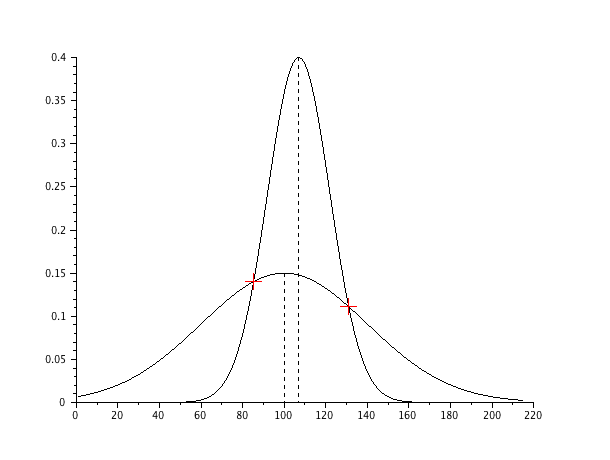
\includegraphics[width=.33\textwidth]{dessin_gauss/gmm_translation1.png}}
\subfloat[Cas limite, $\Delta c = C$]{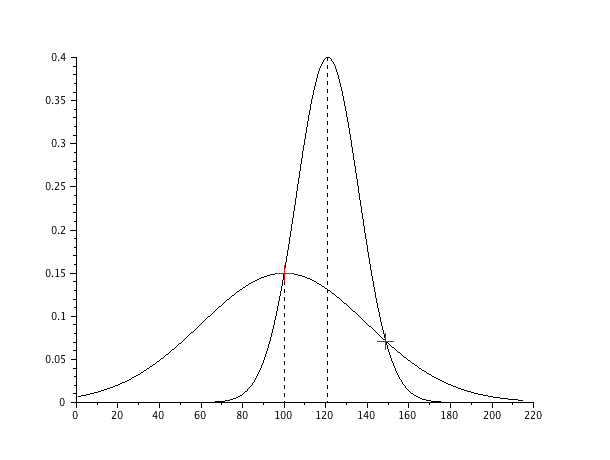
\includegraphics[width=.33\textwidth]{dessin_gauss/gmm_translation2.png}}
\subfloat[$\Delta c >C$]{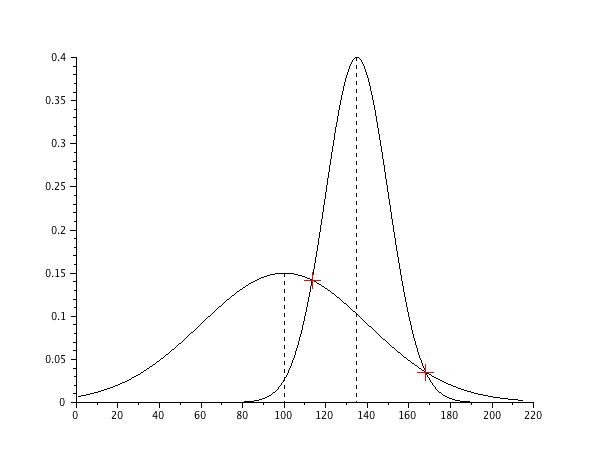
\includegraphics[width=.33\textwidth]{dessin_gauss/gmm_translation3.png}}
\caption{\label{fig:influence_dc} Influence de $\Delta c$ sur la position des points d'intersections (\mbox{$C=\max \left( -2\sigma_1^2 \ln(h_2/h_1) , 2\sigma_2^2 \ln(h_2/h_1) \right)$}).}
\end{figure}
Sur la Figure~\ref{fig:influence_dc}, on peut voir l'influence de $\Delta c$ sur la position des points d'intersections. Le graphique illustre bien le critère donné par le théorème~\ref{thm:anxe_pt_unique}. Ce critère est cependant relativement restrictif.\todo{Graphique de la condition racine intrene ?} On ne peut donc pas compter sur la présence systématique d'un point d'intersection interne pour établir un critère d'\hetero. Peux-t-on au moins espérer avoir toujours 2 points d'intersections ?


\subsection*{Analyse du discriminant.}
Intéressons nous maintenant de plus près au discriminant~\eqref{eq:anxe_discr_reduit}. Pour cela fixons $\sigma_2=a$ et posons $\sigma_1=\sigma$. On a donc à étudier~:
\begin{equation}\label{eq:discr_v2}
\Delta'(\sigma,w,\Delta c) = a^2 \sigma^2 \left[ (\Delta c)^2 + 2(\sigma^2-a^2)\ln\left( \frac{(1-w)\sigma}{wa} \right) \right]
\end{equation}
Remarquons que les points d'annulation de ce discriminant correspondent au ligne de niveaux négatives de la fonction
$$f( \sigma,w ) := (\sigma^2-a^2)\ln\left( \frac{(1-w)\sigma}{wa} \right). $$
Etudions donc la fonction $f( \sigma,w )$.

\begin{figure}
\centering
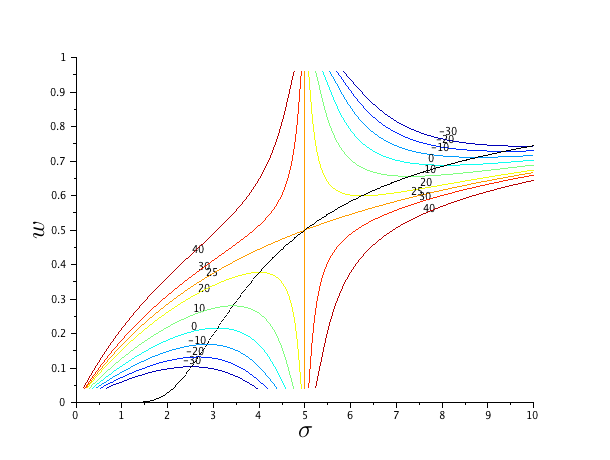
\includegraphics[width=.75\textwidth]{dessin_gauss/discriminant2.png}
\vspace{-5mm}
\caption{\label{fig:courbe_nvx_discrim}Courbes de niveaux du discriminant donné par l'équation~\eqref{eq:discr_v2} -- Ici, $a=5$ et $\Delta c=5$.}
\end{figure}
\paragraph{Points critiques de $f( \sigma,w )$.}
Le gradient de $f$ est donné par~:
\begin{equation}
\nabla f = \begin{pmatrix}
\diff{f}{\sigma} \\ \diff{f}{w}
\end{pmatrix}=\begin{pmatrix}
2\sigma \ln\left( \frac{(1-w)\sigma}{wa} \right) + \frac{\sigma^2-a^2}{\sigma}\\ \frac{a^2-\sigma^2}{w(1-w)}
\end{pmatrix}.
\end{equation}
Ainsi, à $\sigma$ fixé, $\diff{f}{w}$ est toujours du signe de $a^2-\sigma^2$. Il ne s'annule donc jamais. Il n'y a donc pas de point stationnaire. Pour $\sigma$ fixé~:
\begin{itemize}
\item $f$ est croissante si $\sigma < a$
\item $f$ est décroissante si $a<\sigma$
\item $f(\sigma=a, w) \equiv 0$.
\end{itemize}
\paragraph{Lignes de niveaux de $f( \sigma,w )$.}
Soit $w_k(\sigma)$ la ligne de niveau correspondant à $f(\sigma,w)=-k$, avec $k= (\Delta c ^2) /2$. On a donc~:
\begin{align*}
f(\sigma,w)=-k & \Leftrightarrow \ln\left( \left( \frac{1}{w}-1 \right) \frac{\sigma}{a}  \right) = \frac{-k}{\sigma^2-a^2} \\
& \Leftrightarrow w_k(\sigma) = \left[ \frac{a}{\sigma} \exp \left( \frac{-k}{\sigma^2-a^2} \right) +1\right]^{-1}
\end{align*}
Une analyse des variations de $w_k(\sigma)$ permet de tracer l'allure du discriminant, qui est présenté sur la Figure~\ref{fig:courbe_nvx_discrim}.


Les cas où le discriminant est négatif sont donc minoritaire. Ceci explique en partie, qu'en pratique nous n'avons rencontré aucun cas de gaussienne qui ne s'intersectent pas. Construire un critère d'\hetero basé sur la position de ces 2 points (ou de l'un de ces deux points) n'est donc pas insensé.

\end{document}